\documentclass{sig-alternate}
\usepackage{auto-pst-pdf}
\usepackage{graphicx}
\usepackage{multicol}
\usepackage{amsmath}
\usepackage{float}
\usepackage{qtree}
\usepackage{array,hhline}
\usepackage[ruled,vlined]{algorithm2e}

\usepackage{titlesec}

\titleformat*{\subsection}{\normalsize\bfseries}
\titleformat*{\subsubsection}{\normalsize\bfseries}

\graphicspath{ {./assets/} }

\begin{document}

\title{Automatic User Profiling for Intelligent
Tourist Trip Personalisation}
%\numberofauthors{1} %  in this sample file, there are a *total*
\author{
% 1st. author
\alignauthor
Liam Attard\\
       \affaddr{University of Malta}\\
       %\affaddr{Msida, Malta}\\
       \email{liam.attard.18@um.edu.mt}
   }
% 2nd. author
%\alignauthor
%Dr Josef Bajada\\
       %\affaddr{University of Malta}\\
       %%\affaddr{Msida, Malta}\\
       %\email{josef.bajada@um.edu.mt}
%}

\date{12th July 2021}

\makeatletter
\def\@copyrightspace{\relax}
\makeatother

\maketitle
\begin{abstract}

We present a tourist itinerary recommendation
algorithm that assists upcoming tourists by
autonomously generating a personalised holiday plan
according to their constraints. The system
automatically builds a travel interest profile from
the user's social media presence and recommends places
tailored to the user's interests.  Convolutional
Neural Networks (CNN) classify the user's social media
pictures into their respective travel category; Beach,
Clubbing, Nature, Museums, Bars and Shopping. These
determine their predominant travel interest topics.
Then, two meta-heuristics, Particle Swarm
Optimisation (PSO) and Genetic Algorithms (GA) use this
computed travel profile to optimise a personalised
plan. We evaluate the performance based on their plan
quality and performance.The system was packaged into an application that
allows users to connect with their social media
accounts and generate a plan for a holiday in Malta.
We assessed the effectiveness of implementing
automatic personalisation in a holiday planning
application through in-depth semi-structured
interviews by comparing a personalised and a more
generic itinerary.


\end{abstract}


%\keywords{Tourist Trip Design Problem, Particle Swarm Optimisation, 
            %Genetic Algorithms, Convolution Neural Networks}

\section{Introduction}


Leisure travelling is an impactful industry
whose economic importance significantly improves each
year, contributing to 10.4\% of the global GDP in 2019
~\cite{wttc2018travel}. Despite this, planning for a trip to a
foreign city requires a substantial amount of
time-consuming research. As a result, people often
rely on multiple data sources such as travel
brochures, blogs and vlogs to form a holiday plan and
retrieve the top-rated points of interests (POI) of a site. 
However,  these mediums do not hold the
resources to provide POIs tailored according to the traveller's preferences ,and
constraints and a tourist has to compile a timetable
independently
~\cite{DeChoudhury2010}. 

In literature, offering tourists a personalised route
composed of POIs has been defined as the tourist trip
design problem (TTDP). The TTDP comprises ranking
and selecting POIs that might interest the user and
create a feasible plan. 
This is an NP-hard problem where complete 
algorithms only manage to optimise with a small number
of POIs. Therefore, many approximate algorithms,
namely heuristic and meta-heuristic approaches, work
to converge solutions with complex alternatives to
this problem.

Nevertheless, the few existing systems that provide
users with an itinerary or activity plan require a lengthy
process of manually gathering the users' likes and
constraints or information from past trips. 
\\
\\

\noindent  We will try to answer the following research question:


\begin{center}

\textit{Can a system automatically recognise a tourist's travel
preferences and use this information to generate a personalised itinerary
for a holiday?}

\end{center}


%\begin{figure}[h]
%\centering
%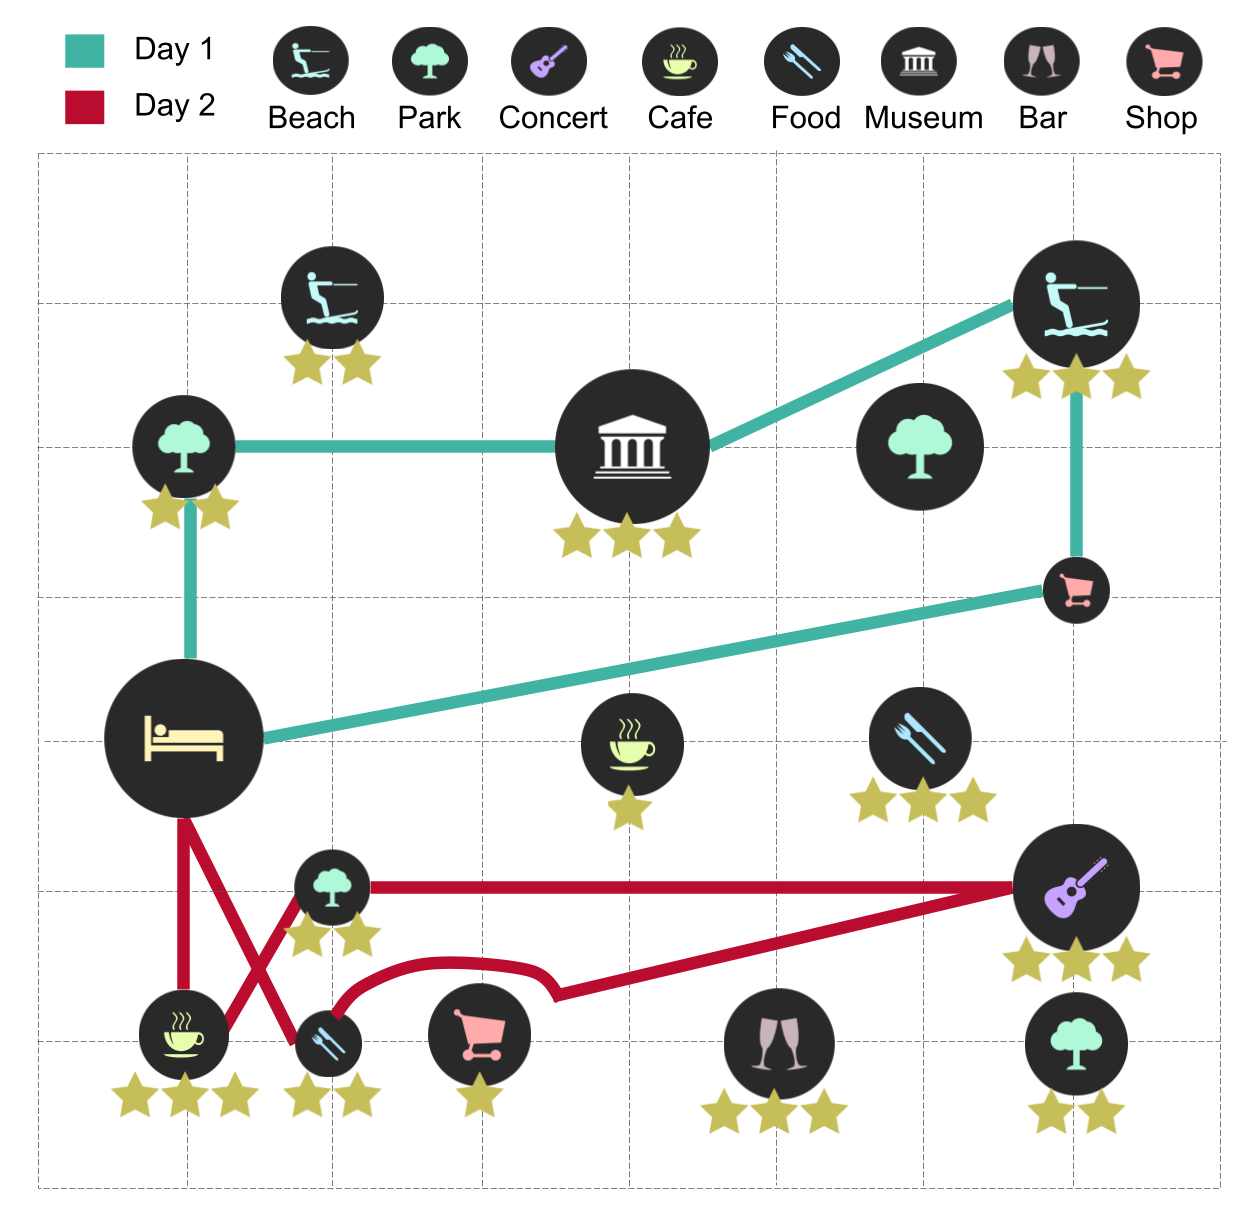
\includegraphics[width=0.4\textwidth]{TTDP.png}
%\caption{Example of a tourist planning problem}
%\label{TTDP}
%\end{figure}



\subsection{Aims and Objectives}

We aim to build an application that
generates a personalised holiday plan according to the
user's travel dates and constraints. The following are the objectives:


\begin{itemize}
    \item \textbf{Objective 1 (O1)}: Investigate techniques to build travel interest
    profiles automatically from social media interactions.  
    \item \textbf{Objective 2 (O2)}: Explore different optimisation algorithms for
    building personalised travel itineraries using the
    generated travel interest profiles. 
    \item \textbf{Objective 3 (O3)}: Evaluate the
    performance of the personalised travel itinerary
    generator with real users through in-depth
    semi-structured interviews. 

\end{itemize}

%We will conduct the interviews by generating a
%personalised and non-personalised timetable for a
%holiday in Malta to have prior knowledge of the POIs
%and compare the effects of both itineraries.




%
To address this problem, we present an application
that helps tourists travel by providing them with a
complete itinerary for their upcoming holiday using
several optimisation algorithms, namely, Genetic
Algorithms (GA) and Particle Swarm Optimisation (PSO).
With the prevalence of social media and data-driven
approaches, we also automate gathering users' POI
desires by scanning their social media profile using
machine learning classification approaches through
Convolutional Neural Networks (CNN).


%Removed results in intro





\section{Background and Literature Review}
\label{Literature}

This section first discusses automatic user profiling to represent travel
preferences, then overview and formalise the TTDP research area.

\subsection{User Preference Gathering}

User profiles are a virtual representation of a user
containing their characteristics~\cite{Cufoglu}. In
addition, some tourist planners make use of such a
technique to personalise the results of their
system. For example, Wörndl et al.
\cite{Worndl2017} required the upcoming tourists to
input their preferences manually by rating six
categories on a scale of 0 to 5: \textit{Sights and Museums,
Night Life, Food, Outdoors and Recreation
 and Shopping}. Including a manual input of user
preferences resulted in high user satisfaction since
their timetable was very customised.


In 2018, Lim et al.\cite{Lim2018a} demonstrated how
implementing personalisation in their algorithm,
PersTours, helped portray real-life scenarios more
accurately. The authors built a system where the
tourist’s level of interest in a specific category is
dependant on their time spent at such POIs, relative
to the average user. First, they gathered information
from the user’s past trips from the social media
platform Flickr. Then, they evaluated their algorithm
using the Root-Mean-Square Error (RMSE), representing
the time deviation of past trips and PersTours results
from Flickr. Although their results show the PersTours
outperforms other applications that use
frequency-based user interest, this approach requires
users to use Flickr and post information about their
past trips on the platform.
 
Nguyen et al.\cite{Nguyen2018} developed an Android
chat application called STSGroup that gathers user’s
preferences and resolves conflicts between tourists by
understanding the messages sent in a group chat. They
provided an example of students travelling to South
Tyrol (Italy), which gathered information such as the
users’ mood and recommended POIs from their
conversations. Other users in the group chat rate
their suggestions through a voting system as the
system uses raking and logistics to calculate
the ideal group preferences in the background. As a
result, 86.7\% of the test users showed satisfaction
with the suggestions.  


The average internet user has gone from being a
passive content absorber to a content producer through
social media. TTDP solutions can use this advantage
and provide a fully automated activity plan based on
the user's characteristics. The following are some
methods for user profiling and information gathering
from the user's social media. 


Instagram has a significant effect on the tourism
industry. Sharing photos of amazing 
influence the way people choose their
POIs\cite{Terttunen2017}. Therefore, a system that
uses tourist's social media photos could infer the
user's preference.

Guntuku et al.~\cite{Guntuku2017} performed an
analysis on the relationship between a user's
characteristics and online images. They found that the
media on the social media profile can predict the big
five personality traits; conscientiousness,
extraversion, neuroticism, agreeableness and openness.
The performance graded by the Pearson correlations
tests were 0.530 and 0.566 for prognosticating
neuroticism and conscientiousness, respectively. 
Therefore, image classification
techniques could aid a preference
gathering system.




\subsection{Single Route and Multi Route Planners}

%This section will analyse existing optimisation techniques for TTDP solutions.
%These include swarm-based, trajectory-based and evolutionary algorithms.
%Gavalas et al.~\cite{Gavalas2014a} classify TTDP variants into two; Systems
%that produce a single route and systems that can handle multiple days. 

%Trip planner applications aim to offer tourists information in a unified and
%centralised manner, providing them with a plan for their trip. Two domains
%develop current applications: methods for obtaining POIs and tour
%recommendation algorithms that create tourist trips \cite{Lim2018a}.

%\begin{figure}[h]
%\centering
%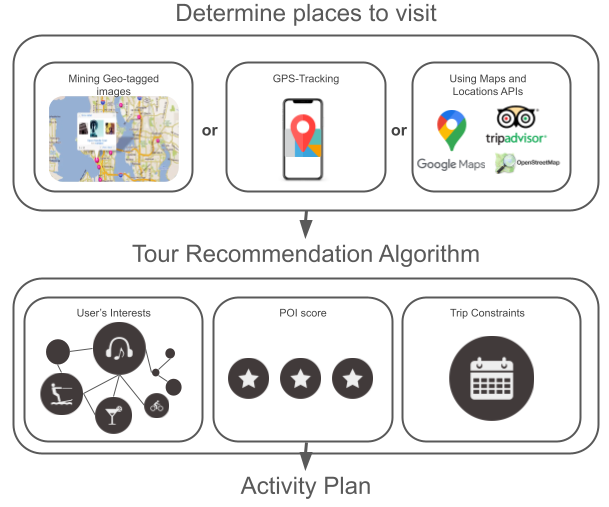
\includegraphics[width=0.4\textwidth]{RSProcess.png}
%\caption{Trip Planner Applications Process.}
%\label{RS}
%\end{figure}

%\subsubsection{Collecting the Points of Interests}

%Before producing an itinerary, the tourist planners have to
%formulate a dataset of POIs from some data source. There are
%several ways to identify an appropriate data source representing
%real-life tourist trajectories. 

%One approach is made by gathering tourist places by mining them from
%geotagged images of Location-Based Social Networks (LSBN) such as Flickr,
%or Facebook~\cite{DeChoudhury2010, Memon2015}.

%A prompt and accurate strategy towards gathering essential places
%in the vicinity uses Mapping \& Location APIs such as 
%Google or TripAdvisor. Worndl et al.\cite{Worndl2017} use this approach and build a
%dataset of prominent POIs by querying their API with the user's
%desired location. In return, they receive a sequence of places and
%information about each site to use as criteria for the itineraries.


%\subsubsection{Single Route Problems}

The Orienteering Problem (OP), introduced by Tsiligirdes
~\cite{Tsiligirides1984}, is the foundation of
single route planners in observance of the sport, orienteering. There are
various types of OPs that include different constraints, such as time windows
and time dependency~\cite{Gunawan2016}. The OP can be represented as a
travelling salesman problem with profits. 

%\setlength{\tabcolsep}{20pt}

Consider a set of POIs \[P = {p_1,p_2,\ldots,p_N}\]
where \textit{p} is a POI having the latitude, longitude, category,
price, and corresponding set of opening hour constraints.
\\
The objective function of OP is:

\[ \text{MAX}  \sum_{i=2}^{N-1} \sum_{j=2}^{N} {s_i}{x_{ij}} \]

\noindent Where \textit{$s_i$} is the score of visiting node \textit{i} and
\textit{$x_{ij}$} is the number of visits by POI \textit{i} followed by POI \textit{j}.

\noindent \paragraph{Constraints:} 

\begin{multicols}{2}
\begin{equation} 
    \label{constraintOne}
    \sum_{j=2}^{N} p_1j = \sum_{i=1}^{N-1} p_{iN}= 1
\end{equation}

\begin{equation} 
    \label{constraintTwo}
    \sum_{i=1}^{N-1} \sum_{j=2}^{N} t_{i}x_{ij}<= Tmax
\end{equation}


\end{multicols}

%\begin{multicols}{2}

\begin{equation} 
    \label{constraintThree}
    \sum_{i=1}^{N-1} x_{ir} = \sum_{j=2}^{N} x_{ij} \geq 1 \, \text{\small{r = 2, \ldots, N-1}}
\end{equation}

\begin{equation} 
    \label{constraintFour}
    2 \geq u_i \geq N 
\end{equation}
%\end{multicols}

\begin{equation} 
    \label{constraintFive}
    u_i - u_j + 1 \geq (N-1)(1-x_{ij})
\end{equation}

where:

\begin{tabular}{l l}
\textit{$t_{ij}$} & travel time from i to j \\
\textit{T} & maximum time \\
\textit{$u_i$} & position of POI i in route\\

               & \\

\end{tabular}


Constraint~\ref{constraintOne} ensures that the path starts at POI 1 and ends at POI N.
Constraint~\ref{constraintTwo} limits the total travel time.
Constraint~\ref{constraintThree} ensures that each POI is visited only once.
Constraint~\ref{constraintFour} and constraint~\ref{constraintFive} ensure no subtours.
\\


%\begin{figure*}[h]
%\Tree [.{Orienteering Problem (Single Route)} .{Op with Time Windows}  {Time-Dependent OP} 
%{Team OP (Multi-Route)} !{\qframesubtree} ]
%\caption{Some Variants of the Orienteering Problem}
%\label{variants}
%\end{figure*}

There are numerous Evolutionary Algorithms (EA) proposed to solve OP.\@
~\cite{Kobeaga2018,Wang2008}. EAs are algorithms based on natural evolution which
use a fitness score to get to the best solution of a problem, in this case, the
TTDP~\cite{Gunawan2016}.


%\centering
%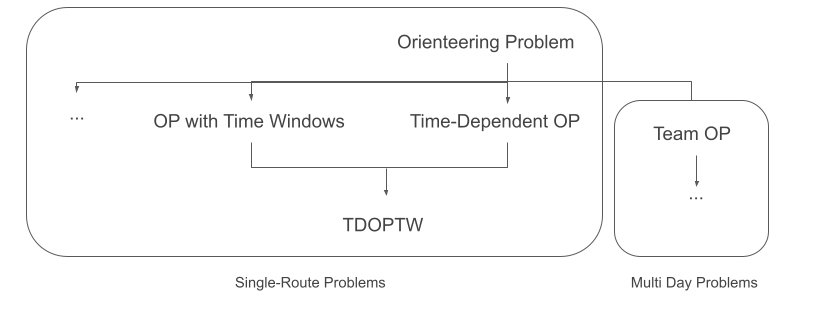
\includegraphics[width=0.5\textwidth]{TOP_graph.png}

Particle Swarm Optimisation-based (PSO) systems provide prevalent OP solutions
with fast computing time~\cite{Yu2019}.  Sevkli
et al.~\cite{Sevkli2010,Sevkli2010a} tested out two PSO variants:
Strengthened Particle Swarm Optimization (StPSO) and Discrete Strengthened
Particle Swarm Optimization (DStPSO). These two algorithms introduce pioneering
particles, which first perform a local search-based technique called Reduce
Variable Neighborhood Search (RVNS) between all the particles and then assign a
random velocity. These PSO algorithms obtains either the best or competitive
solutions compared with other algorithms such as Ant Colony and Genetic
Algorithms when tested on the Tsiligirides~\cite{Tsiligirides1984, Chen2011a}
dataset of predefined nodes.

A novel approach in 2018  by Kobeaga et al.~\cite{Kobeaga2018} was able to
achieve competitive solutions for medium-sized instances of over 400 nodes and
find new best-known solutions for large datasets using the steady-state genetic
algorithm. The algorithm also implements a local search, which aims to reduce
travel time. Santini et al.~\cite{Santini2019} introduced a heuristic algorithm
based on adaptive extensive neighbourhood search. When they evaluated their
system, results showed that EA solutions such as the Kobeaga's GA~\cite{Kobeaga2018} found slightly more suitable
solutions, while their algorithm had a lower average gap between many
solutions.

In real-life scenarios, POIs have time constraints that allow them to be
visited only during specific hours, such as opening and closing hours or public
holiday constraints. Traditional OP is not able to cater for such problems. A
single route variant of the OP which solves these issues is the Orienteering
Problem with Time Windows (OPTW)~\cite{Gavalas2014a}. 

Kantor et al.~\cite{Kantor1992} provided the first attempt towards the
OPTW~\cite{Vansteenwegen2011}. They developed two algorithms;
Insertion and depth-first search. The former algorithm solves the path by
selecting a POI with the highest score over-insertion cost incrementally. On
the other hand, the depth-first search algorithm gathers parallel tree-based
solutions simultaneously and iteratively adds new POIs as long as they follow a
set of constraints. Their evaluation showed significant improvements of the
second algorithm over the insertion. 

When travelling between two POIs, the travel time may depend on certain
variable time constraints such as the traffic levels and waiting time~\cite{Herzog2020}.
The Time-Dependent Orienteering Problem (TDOP) introduced by Fomin et al.
~\cite{Fomin2002} is the single route variant of OP, which considers
these scenarios since traditional OPand OPTW does not~\cite{Gunawan2016}. In 2011, Abbaspour et
al.~\cite{Abbaspour2011}provide a solution for the
Time-Dependent Orienteering Problem with Time Windows, which combines the two
previously mentioned OP variants \\(TDOPTW).  They propose two adaptive genetic
algorithms and multi-modal shortest pathfinding evaluated in the city of
Tehran.


%\subsubsection{Multiple Route Problems.}

The solutions available from what we discussed in the previous sections can only
generate a single efficient path for a tourist's holiday. The Team Orienteering
Problem (TOP)~\cite{Chao1996} is a variant of the OP, which allows for
solving the TTDP with multiple days~\cite{Sylejmani2017}. The system generates a full
itinerary for the tourist, with a maximum total score of all routes~\cite{Herzog2020}.

Several solutions use PSO-based algorithms to solve the TOP.
Muthuswamy et al.~\cite{Muthuswamy2011} developed a discrete version of the PSO (DPSO)
which can generate n routes where $2 \geq n \geq 4$. The algorithm consists of two procedures;
Random initialisation of n-1 routes. The n\textsuperscript{th}
route is based on partial randomness and the current score divided by the current
distance of each particle after updating the velocity.  The
particles use RVNS and 2-opt techniques to communicate with each other as local
search techniques. The authors evaluated their work by comparing the algorithm
to seven TOP heuristics in which DPSO performed competitively across all
applied benchmark data sets~\cite{Gavalas2014a}.

A few years later, Dang et al.\ wrote another PSO inspired algorithm (PSOiA) for
the TOP.\@ They evaluated their work using an interval graph model, which showed
how to examine a more extensive search space faster~\cite{Gunawan2016}.

Besides swarm-based algorithms, an algorithm by Sylejmani et al.~\cite{Sylejmani2012}
used the trajectory-based tabu search to solve a Multi Constrained Team OPTW.\
Their system followed three steps in order to generate an activity plan: a new
activity is added as a node to the trip using \emph{Insert}, a node is
exchanged with a new activity using \emph{Replace} and two nodes swap with each
other using \emph{Swap}. 



\subsection{Conclusion}
We have concluded that it is possible to gather characteristics from social media throughout this
research. Therefore, we will introduce this technology to generate user
profiles as part of a constraint with the objective function of the
optimisation algorithm.

Since the evolutionary algorithms, PSO and GA, resulted in competing solutions
on the Tsilgidres Dataset and are used in novel solutions~\cite{Yu2019,
Wisittipanich2020}, we will compare both algorithms to see which one to use as
the baseline for our TDOPTW application.





\section{Methodology}
\label{MethodologyPage}

This section will elaborate user-profiling methods, 
the itinerary generator and the implementation used to build this application.
Figure~\ref{Methodology} outlines the overall process of our personalised
itinerary generation
framework. 

\begin{figure}[h]
\centering
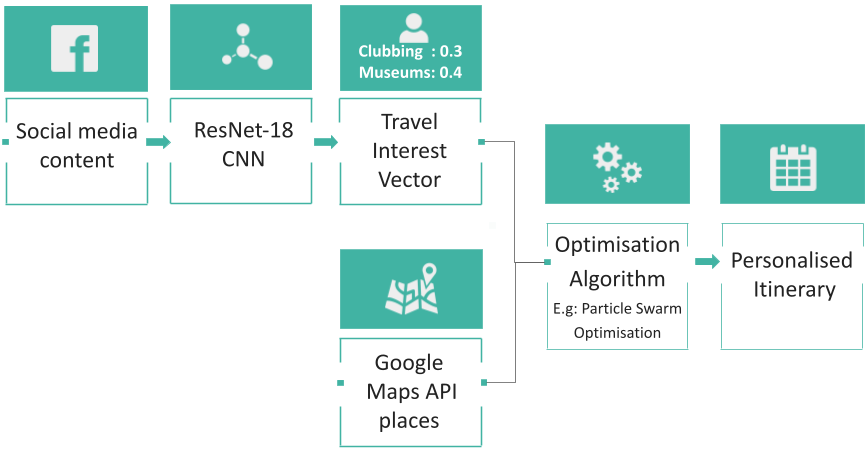
\includegraphics[width=0.5\textwidth]{Methodology.png}
\caption{Personalised itinerary generator}
\label{Methodology}
\end{figure}

\subsection{Generating the User Profile}

Many people are present on social media posting
pictures of their travel moments~\cite{Miller2016}. For this reason, we opted to
build a user profile from the user's online presence. A travel interest vector is made up a vector of six integer values
\[<v_0, v_1, v_2, v_3, v_4, v_5>\] representing the user profile.
Each element represents the following POI categories 0 Beach,1 Nature,2
Shopping,3 Museums,4 Clubbing and 5 Bars.
    

At the start of the application, the
travel interest vector is initialised with zero
values, and the app increments a category whenever the
user's content matches. $v_0$ to $v_3$ represents morning categories
and $v_4$, $v_5$ represent evening categories. After
the data collection process is complete, the
vector values are normalised independently. 

Facebook's API that allows users to connect Facebook
and Instagram accounts and request content from the user with their permission.
The app requests the photos and the liked pages used to 
populate the user's travel interest
vector. 

\noindent \textbf{Transforming the liked pages into the travel interest vector: } The API's documentation contains a whole list of possible
page categories. 
%TODO: Add Url
%https://www.facebook.com/pages/category. 
The app iterates through all of these user's liked
page categories and increments a value in the travel
interest vector whenever the Facebook result matches.
For example, if a user likes a page with class `DJ',
the user's clubbing vector value is incremented, and if a page is labelled as a
`Mountain', increments the user's nature vector value.

\noindent \textbf{Transforming the user's photos into the travel interest
vector} Convolutional Neural Networks have become a standard
for classifying an image because of their high
accuracy~\cite{Zhou2018}. Therefore, we decided to test
out two approaches for classifying the photos into the
app's six categories. 

Zhou et al. \cite{Zhou2018} trained several CNNs for
scene recognition and generic deep scene features for
visual identification. However, the places365 models
are not explicitly trained on the six categories of
our application. Therefore, we need to carefully map
the 365 categories with our six application's
categories. That is why we introduced a Tensorflow
Keras sequential model, explicitly trained on the six
application's categories to compare.

The pretrained places365 models are 
pretrained models trained on the places365-standard dataset of about
1.8 million images to classify an image into 365
different scene categories. We used the Resnet
places365 models, Resnet-18 and Resnet-50 since they
achieved the highest top-5 validation accuracy on the
places365 dataset. The Resnet 18 comprises 18, and the
Resnet 50 comprises 50 convolutional layers. They both
converge to an output layer representing the 365
output categories.

The Tensorflow Keras sequential model 
contains three convolutional layers with a
rectified linear unit (ReLu) activation function. A
pooling layer follows each to lower the input volume's
spatial dimension for the upcoming layers. The first
layer is a rescaling layer that resizes an image to
180$\times$180 pixels. The final layer represents a
flattening layer and two dense layers to reduce the
outputs to the six application categories, and another
representing `None'.

The dataset contains 3600 public internet images
representing the seven classes: Beach, Nature,
Museums, Shopping, Clubbing and Bars and None. The
tensor library provides tools to Split the dataset
into a training and validation set Distribute the
photos into batches of 32 Cache the dataset to memory
to prevent I/O blocking All of the images were resized
to 180x180 pixels, and the RGB values were normalised
from zero to one.  	Since the dataset is small
compared to the places 365 models, the training
process is prone to overfitting. Data augmentation
generates additional samples using random
transformations on the dataset. We also added
a dropout layer to the model randomly drops sets the
input values of the neuron. These two techniques help
the model avoid overfitting.

%\begin{figure}[h]
%\centering
%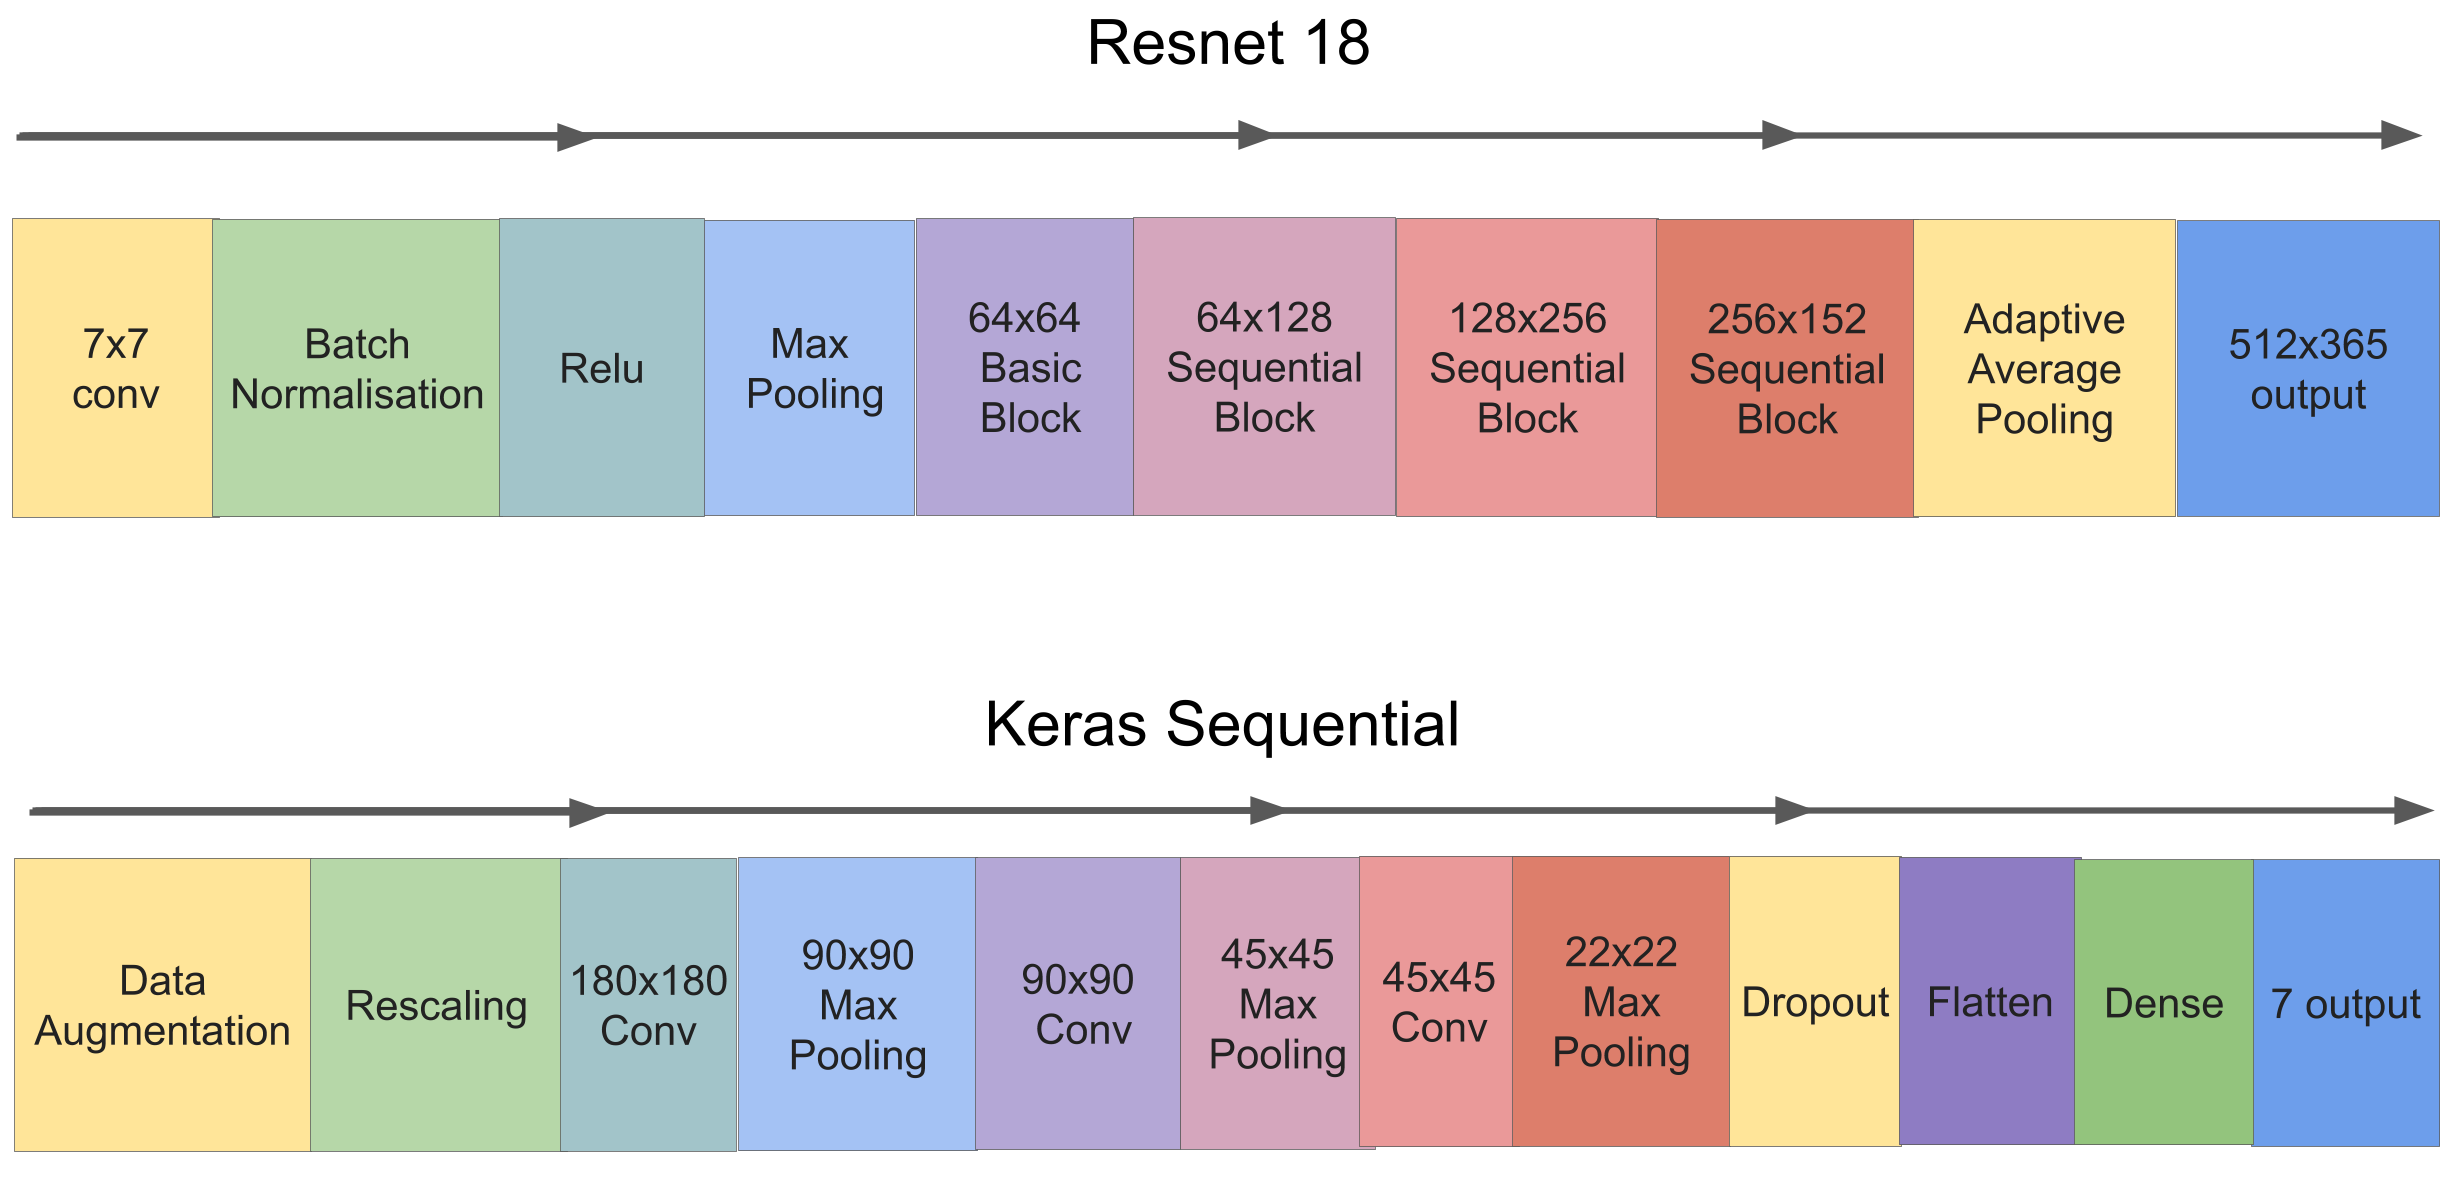
\includegraphics[width=0.55\textwidth]{Models.png}
%\caption{Model Architectures}
%\label{Models}
%\end{figure}






\subsection{Producing the activity plan}

The problem of our itinerary planner algorithm
is mathematically formulated as follows. A tourist trip is made up
of some pre-defined user constants alongside the travel interest
vector. The predefined constants are:
\\
\setlength{\tabcolsep}{20pt}

\begin{tabular}{l l}

\textit{M}:  &  The number of travelling days. \\
\textit{C}: & The activity pace.\\  
\end{tabular}
\\
\\
The objective function of our itinerary planner is:

\[ \text{MAX}  \sum_{m=0}^{M} ( S_{{D_m}} + S_{{E_m}}) \]
where:
\\
\begin{tabular}{l l}
% \textit{i,j}:  &  POI (\textit{i,j} = 2,3,...,\textit{N}) \\
\textit{m} & Travelling day (\textit{m}=1,2,\ldots, \textit{M}) \\ 
\textit{$D_m$} & Morning section of day number m \\  
\textit{$E_m$} & Evening section of day number m \\  
\textit{$S_{D_m}$} & Score of the morning section $D_m$ \\  
\textit{$S_{E_m}$} & Score of the evening section $E_m$ \\  
\end{tabular}
\\
\\

A day is made up of the morning ${D_m}$ section and
the evening ${E_m}$ section. The timetable suggests a
POI in the morning, then somewhere to eat, and the
rest is dependant on the activity pace C. That is why
the morning section is made up of $C + 2$ tourist
attractions. The evening section suggests a place to
eat and a POI; therefore, the evening section is just
made up of $2$. 

\begin{center}
$D_m = Y_i + Y_f + C ( Y_i)$ and $E_m = Y_f + Y_j $

\end{center}



\begin{tabular}{l l}

\textit{i} & Morning attraction (i = 1,…, $n_1$)\\
\textit{j} & Evening attraction (j = 1,…, $n_2$)\\
\textit{f} & Food Place (f = 1,…, $n_3$)\\
\textit{$Y_{i|f|j}$}: & Number of times POI is visited. \\
\end{tabular}
\\ 
\\
\begin{tabular}{l l}
\textbf{Constraints} & \\
\textit{$ \sum_{m=0}^{M}\sum_{i=0}^{n_1}{Y_i} \leq 1$} & Ensures morning POIs\\ & not visited more than once. \\

\textit{$ \sum_{m=0}^{M}\sum_{j=0}^{n_1}{Y_j} \leq 1$} & Ensures evening POIs\\ & not visited more than once.\\


\end{tabular}

The score $S_{D_m}$ or $S_{E_m}$ is calculated using

\[ S_{D_m | E_m} = \frac{1}{T} + R + V\]

where:
\\
\begin{tabular}{l l}
% \textit{i,j}:  &  POI (\textit{i,j} = 2,3,...,\textit{N}) \\
\textit{T} & Distance between POIs of day m\\ 
\textit{R} & Average rating of POIs of day m\\  
\textit{V} & How much POIs match with the \\ &  user's travel interest vector. \\  

\end{tabular}
\\



\begin{algorithm}[h]

 iter = x \;
 count = 0 \;
 particles = RandomBiasInitialiser(); \;
 bestParticle = particle[0] \;

 \While{count $>$ x}{

     i = 0 \;
     maxScore = 0 \;

     \While{i $<=$ particles.length}{

         \tcc{Updating personal best}
        \If{particles[i].score $>$ particles[i].personalBest.score}{

             particles[i].personalBest = particles[i].position\;

         }

         \tcc{Updating global best}
        \If{particles[i].score $>$ maxScore}{


             maxScore = particles[i].score \;
             bestParticle = particles[i].position \;

         }

         i = i +1 \;

         \tcc{Calculate new position}
         particle[i].calculateNewPosition() \;



     }
     \Return bestParticle

 }

 \caption{Particle Swarm Optimisation}
    \label{PSOAlgorithm}
\end{algorithm}



%\subsubsection{}
\subsubsection{Optimisation Algorithms}

PSO and GAs are two meta-heuristics that use a population
to converge to a fit solution. Therefore, they require
an initial random generation of possible timetables. In
our algorithm, we introduce a method of randomisation
bias. With this technique, the randomness of the initial
population is weighted based on the place's rating and 
the place's number of ratings. This bias gives a 
head start to the algorithm rather than just starting 
optimising from purely random itineraries, highly likely 
to be of bad quality.

%\begin{algorithm}[h]

 iter = x \;
 count = 0 \;
 particles = RandomBiasInitialiser(); \;
 bestParticle = particle[0] \;

 \While{count $>$ x}{

     i = 0 \;
     maxScore = 0 \;

     \While{i $<=$ particles.length}{

         \tcc{Updating personal best}
        \If{particles[i].score $>$ particles[i].personalBest.score}{

             particles[i].personalBest = particles[i].position\;

         }

         \tcc{Updating global best}
        \If{particles[i].score $>$ maxScore}{


             maxScore = particles[i].score \;
             bestParticle = particles[i].position \;

         }

         i = i +1 \;

         \tcc{Calculate new position}
         particle[i].calculateNewPosition() \;



     }
     \Return bestParticle

 }

 \caption{Particle Swarm Optimisation}
    \label{PSOAlgorithm}
\end{algorithm}




%\paragraph{Particle Swarm Optimisation}

In PSO, the whole population is referred to as the
swarm, whilst a single member a particle in this case representing a timetable
solution. Each particle uses its current position, personal best and global best
to calculate its new position. After a few iterations have passed, particles use
their velocity and move towards the optimum position.
We demonstrate the framework of our PSO algorithm in
algorithm \ref{PSOAlgorithm}.


%\paragraph{Genetic Algorithms}

Genetics algorithms use biological terms to describe
their attributes. For example, a timetable solution in
population is referred to as a chromosome~\cite{Abbaspour2011}. 

In PSO, the algorithm optimises by allowing each
particle to move closer to the global best every
iteration. In comparison, in GAs, first, the best
chromosomes known as the elites are selected from each
iteration. Then, three techniques, namely selection,
mutation, and crossover, are applied to generate the
next population.

We used the geneticalgorithm2 package~\footnote{https://pypi.org/project/geneticalgorithm2/},
which allowed us to use the same score function and
the random bias to initialise the particles. The
algorithm has 7 parameters. The parents portion
represents the number of parents who will reproduce
and create the next generation. The mutation
probability determines the chance a POI in a
chromosome will be replaced by a random value to which
the algorithm will converge less quickly and explore
more of the search space. The crossover probability
will affect the chance that part of its solution goes
to the child. Finally, the elite ratio determines how
much of the best chromosomes in an iteration make it
to the next iteration.  There are many types of
crossovers techniques. In this algorithm, we
explored \textit{one point, two point, uniform and shuffle crossover}.  The algorithm produced the following
steps: \\
\textbf{Step 1}: Initialise the first population using random bias. \\
\textbf{Step 2}: Select the best chromosomes from the population. \\ 
\textbf{Step 3}: Select the elite particles that will make it to the next iteration.\\
\textbf{Step 3}: Apply Crossover, Mutation and Selection on the population. \\
\textbf{Step 4}: Check if the number of iterations has exceeded. 







\section{Results and Evaluation}

This section will evaluate the image classification technique for automatic user profiling, the itinerary
generation algorithm and the performance of the
whole application and its effects through the interviews.



\subsection{Automatic User Profiling}

We trained the Keras Sequential model using the NVIDIA
Tesla K80 GPU provided by Google Colab. At 16 epochs,
the model starts to overfit as the validation loss
starts to increase. The testing dataset consists of
500 images manually gathered using the Unsplash API. 


When comparing the Resnet 50, Resnet 18 and Keras
Sequential model,the Reset 50 achieved the best
average accuracy, precision and recall. The resnet 50 achieved the highest F1 score the
on testing dataset with an average F1 score of 76.29. So
we decided to use it as our baseline for the tourist
itinerary generation application.

\begin{figure}[h]
\centering
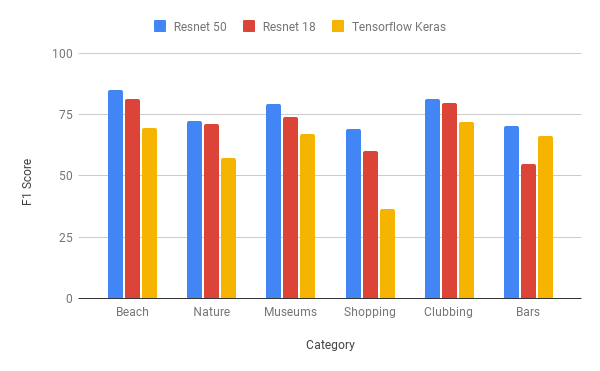
\includegraphics[width=0.45\textwidth]{F1Score.png}
\caption{F1 score of the three models}
\label{f1}
\end{figure}



\subsection{Itinerary Optimisation Algorithms}

We generated 50 random constraints and tested them out
on the PSO and GA algorithm. Figure~\ref{AverageScore} shows how the number of
particles affects the score. For 100 population
members, both algorithms achieve similar average
scores. However, the difference in score is not
proportional to the average time taken to complete a
single day, as shown in figure ~\ref{AverageTime}. Since other users will use
the application, we did not
want the generation's time to affect the user
experience. The difference between the average
score of 50 and 100 particles for PSO is only 0.5,
this variant provides the best balance of time and
score so it chosen for our
application.   


\begin{figure}[h]
\centering
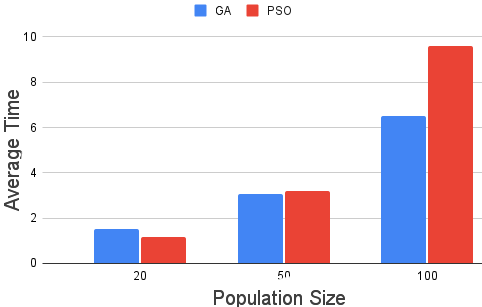
\includegraphics[width=0.3\textwidth]{AverageTime.png}
\caption{Average time spent for 50 iterations}
\label{AverageTime}
\end{figure}

\begin{figure}[h]
\centering
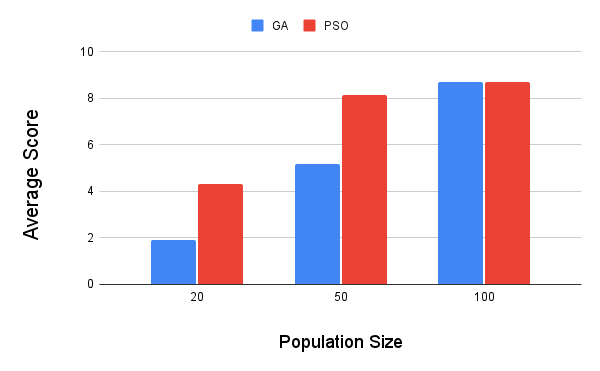
\includegraphics[width=0.3\textwidth]{AverageScore.png}
\caption{Average score achieved for 50 iterations}
\label{AverageScore}
\end{figure}

\subsection{In-depth Semi-structured Interviews}

From all of the twenty interviews, fifteen people preferred the personalised
itineraries and gave valid reasons. However, three out of the people who
selected the non-personalised itinerary stated that they think their social
media presence does not reflect their travel preferences.


%\paragraph{Inidividual one}:  
%The first interviewee had the following traits: personal characteristics:
%enjoys shopping, nightlife and clubbing. Since they do not like to miss out on
%any POIs of a site, they chose to generate a fast-paced activity plan $C = 3$ for
%seven days $M = 7$. Person one is active on social media and posts frequently on
%social media. The application gathered 100 preferences from this person, and
%table ~\ref{indOne} shows their generated travel interest vector.
									
%The first timetable shown was the non-personalised itinerary, and they made the
%following points:

%\begin{table}[h]
%\caption{Travel Interest Vector of Individual One} \label{t:tab}

%\centerline{
  %\begin{tabular}{|l|c|c|c|c|c|} 
 %\hline
      %Beach & Museums	& Nature	& Shops & Clubs & Bars \\
 %\hline
      %1.32\% & 4.35\%	& 4.61\%	& 89.47\% & 69.23\% &30.77\%\\
 %\hline
  %\end{tabular}
%}
%\label{indOne}
%\end{table}

%\begin{itemize}
%\item Initially, they thought the timetable was quite personalised since it tried to capture a balance of POIs of a different category and thought this reflected their lifestyle.
%\item They were satisfied with the travel time between the places making it very doable.
%\item They felt that the timetable included too many cultural places and stated that they would change about 40\% of the timeline if they had to follow it strictly and spend more time shopping.
%\item They rated the itinerary as 'quite personalised' and were 'very satisfied'.
%\end{itemize}

%The following are comments from the second itinerary, i.e. the personalised one:
%\begin{itemize}
%\item The interviewee changed their opinion immediately and figured out this was the personalised solution since the first day was a day dedicated to shopping. 
%\item Since the timetable included more natural locations, they felt that this was the appealing itinerary and would stick with 95\% of this plan.
%\item The suggested places were all places that the person has been to recently.
%\item The evening places were very appealing since it includes a lot of the best night clubs.
%\item They rated the itinerary as 'very personalised' and were 'very satisfied'.
%\end{itemize}
%When shown their automatically generated preferences, person one felt that the
%'beach' category should be higher, and the rest was very accurate. In addition, person one deemed this approach ideal since it gives an in-depth itinerary for a tourist, which is also ideal to discover new places.


%\paragraph{Individual two}: 

%When travelling, the second individual searches for a relaxed holiday with a
%mix of beaches and the main tourist attractions. Therefore, they chose to
%generate a moderate activity plan $C=2$ for five days $M=5$.Furthermore, person two thinks
%that their social media presence represents their travel preferences since they
%post numerous pictures when they travel. The application gathered ten pictures
%and liked pages from their profile, and table ~\ref{inTwo} shows the generated preferences.


%\begin{table}[h]
%\caption{Travel Interest Vector of Individual Two} \label{t:tab}

%\centerline{
  %\begin{tabular}{|l|c|c|c|c|c|} 
 %\hline
      %Beach & Museums	& Nature	& Shops & Clubs & Bars \\
 %\hline
      %50\% & 20\%	& 25\%	& 0\% & 0\% &100\%\\
 %\hline
  %\end{tabular}
%}
%\label{inTwo}
%\end{table}

%The first timetable shown was the
%non-personalised itinerary, and they made the following points:
%\begin{itemize}
%\item The holiday is structured very well and reflects their potential travel plan since there is a resting time between the evening activities and a place to eat right after.
%\item They were unsure whether the first itinerary is personalised since they usually spend more time at the beach and less time in Museums.
%\item There are too many clubs in the evening and would personally go to more bars and relaxed places.
%\item They rated this itinerary `not very personalised' but rated 'satisfied' overall. 

%\end{itemize}
%The following are comments from the second itinerary, i.e. the personalised one:
%\begin{itemize}
%\item This itinerary is more personalised since there are more beaches and natural places.
%\item The evenings are more adapted since there are more places to sit down, drink, and chat than clubbing venues.
%\item This itinerary was rated `very personalised' and `very satisfied' overall. 
%\end{itemize}

%After the second itinerary, we discussed the travel interest vector with the
%interviewee. They stated that they would leave their characteristics the same,
%however, switch the shopping category with museums which are preferential. They
%mentioned that the museums category score is a quite high since they like to
%view science-related locations to keep up to date but the number of museums
%presented was deemed to be too high compared to their likings. Six other
%interviewees also mentioned that their ’museums’ characteristic was rated high.

%To further personalise the itinerary, person two suggested that the algorithm
%should also look at the photos posted by the people they follow online since it
%would gather much more information. 

%To personalise the itinerary further, person two suggested that the algorithm
%should also include photos posted by people they follow online, since it would
%gather more information, making the itinerary more accurate.

%\paragraph{Person Three}: When travelling, they tend to look for places with a
%lot of nature and cultural sightseeing. In addition, this person is very
%interested in music and art, so they also like to travel to art galleries and
%museums.  Person three likes to make the most out of their holiday, so they
%chose to generate a fast-paced $C=3$ six-day itinerary $M=6$. However, they don't think
%their social media profile represents what they would look for in a holiday. As
%a result, the application only gathered ten items, and their preferences are as
%follows:

%The first result shown to this person was the personalised itinerary, and
%they made the following conclusions: 

%\begin{table}[h]
%\caption{Travel Interest Vector of Individual Three} \label{t:tab}

%\centerline{
  %\begin{tabular}{|l|c|c|c|c|c|} 
 %\hline
      %Beach & Museums	& Nature	& Shops & Clubs & Bars \\
 %\hline
      %42.86\% & 9.09\%	& 23.81\%	& 23.81\% & 50\% & 50\%\\
 %\hline
  %\end{tabular}
%}
%\label{inTwo}
%\end{table}

%\begin{itemize} 
    %\item They would enjoy
    %less nightlife and more relaxed activities in the evening.  
    %\item They would prefer 
    %more natural sights along with the museums such as hikes and walks around
    %the environment.  
    %\item They felt that the timetable was not very personalised.
    %\end{itemize} 

%From the non-personalised itinerary, person three made the
%following conclusions:

%\begin{itemize} \item They felt that this timetable was more balanced 
%and appropriate.  \item Since it included more
%nature-related places, it felt more personalised.  \end{itemize}

\begin{figure}[H]
\centering
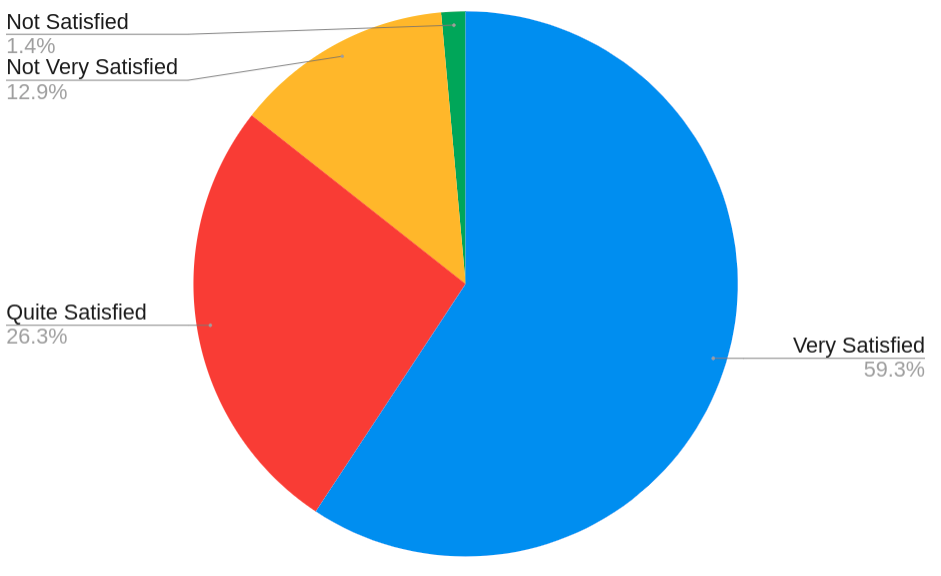
\includegraphics[width=0.34\textwidth]{xiHaga.png}
\caption{Satisfaction Rating of The Gathered Characteristics.}
\label{Satisfaction}
\end{figure}

It was noted that the more active a person is on
social media, the more precise the characteristics are, which leads to a more
reliable travel itinerary. From all of the characteristic categories, seven
interviewees mentioned that their 'museums' category was deemed too high
compared to their liking. They like to follow science-related online content
but do not usually visit many museums when on holiday. Figure
~\ref{Satisfaction} shows that most of the preferences gathered belong to users
who felt very satisfied with the overall results.







\section{Conclusion and Future Work}

We have introduced an automatic preference gathering technique to a TTDP
solution that produces an activity plan through the user's social media photos
and pages they follow. As a result, the system can produce personalised results
within a few seconds. An additional approach targets individuals who do not
feel their online presence represents their travel preferences, such as
gathering using Natural Language techniques to scan the user's text posts.
Although there is always room for further development, we form the basis to
show how an automatic preference gathering system can further assist a
travel application to achieve satisfactory results.



\bibliographystyle{acm}

\bibliography{/home/liam/Documents/latex/library/bibFile/library.bib}

\end{document}


